\documentclass[tikz,border=0pt]{standalone}
\usepackage{xcolor}
\usetikzlibrary{calc}
% Palette: Sam_Comm_final.png by eye, and data/palette.json.
\definecolor{ink}{HTML}{3B2340}
\definecolor{sky}{HTML}{EFC46A}
\definecolor{skyhi}{HTML}{F5DA92}
\definecolor{skylow}{HTML}{E9B060}
\definecolor{cloud}{HTML}{F2D58A}
\definecolor{wallA}{HTML}{E88A73}
\definecolor{wallB}{HTML}{EE9F7E}
\definecolor{wallC}{HTML}{E47A7E}
\definecolor{wallD}{HTML}{F0B07E}
\definecolor{wallE}{HTML}{D9765F}
\definecolor{wallF}{HTML}{E99A8A}
\definecolor{greenA}{HTML}{8DBB7E}
\definecolor{greenB}{HTML}{6FA77A}
\definecolor{greenC}{HTML}{A9C97F}
\definecolor{greenD}{HTML}{5E9C6A}
\definecolor{window}{HTML}{F6E7A0}
\definecolor{windark}{HTML}{8C5A64}
\definecolor{metal}{HTML}{8D9A93}
\definecolor{metaldark}{HTML}{5E6B66}
\definecolor{wood}{HTML}{B9835A}
\definecolor{paving}{HTML}{E2BD8C}
\definecolor{ground}{HTML}{D3A77D}
\definecolor{stone}{HTML}{E7C9A0}
\definecolor{clock}{HTML}{F8EBC8}
\definecolor{court}{HTML}{9E4F55}
\definecolor{courtdark}{HTML}{6E3542}
\definecolor{goldtrim}{HTML}{F2B53A}
\definecolor{paper}{HTML}{F6E7C4}
\definecolor{paperdark}{HTML}{E3CC98}
\definecolor{violet}{HTML}{7B2FF7}
\definecolor{magenta}{HTML}{FF2E88}
\definecolor{cyan}{HTML}{13CFE3}
\definecolor{gold}{HTML}{FFB000}
\definecolor{coat}{HTML}{2F4858}
\definecolor{coatdark}{HTML}{22323F}
\definecolor{trim}{HTML}{F26B38}
\definecolor{skin}{HTML}{E0AC69}
\definecolor{hair}{HTML}{3B2340}
\definecolor{gun}{HTML}{3E3A46}
\definecolor{robe}{HTML}{2D2240}
\definecolor{bossface}{HTML}{F8EBC8}
\definecolor{eye}{HTML}{FF2E88}
\definecolor{red}{HTML}{B3262E}
\definecolor{heart}{HTML}{FF4F6D}
\definecolor{jump}{HTML}{8DE36B}
\definecolor{lamp}{HTML}{FFE6A3}
\definecolor{night}{HTML}{4A3357}
\definecolor{nightsky}{HTML}{6B4A6E}
\definecolor{icesky}{HTML}{A7C4E2}
\definecolor{icefog}{HTML}{8FAFD2}
\definecolor{icesnow}{HTML}{EEF5F9}
\definecolor{icesnowdark}{HTML}{CFDDE7}
\definecolor{icewhite}{HTML}{E4F1F8}
\definecolor{iceblue}{HTML}{A9D3EA}
\definecolor{icedeep}{HTML}{6FA9D2}
\definecolor{iceglow}{HTML}{8FE3FF}
\definecolor{icerock}{HTML}{5E6E82}
\definecolor{icerockdark}{HTML}{3F4C5F}
\definecolor{icered}{HTML}{D94A3A}
\definecolor{hull}{HTML}{A8392F}
\definecolor{hulldark}{HTML}{6C2A27}
\definecolor{icemetal}{HTML}{8A97A6}
\definecolor{canvas}{HTML}{E9C47C}
\definecolor{auroragreen}{HTML}{5CF2B0}
\definecolor{aurorapink}{HTML}{F27AD0}
\definecolor{cobalt}{HTML}{1F4FFF}
\definecolor{ember}{HTML}{FF6A1A}
\definecolor{witnessrobe}{HTML}{1E2742}
\definecolor{witnessice}{HTML}{CDEBFA}
\definecolor{navy}{HTML}{1C2A44}
\definecolor{water}{HTML}{2C6690}
\definecolor{dawn}{HTML}{F7C89A}
\definecolor{housesky}{HTML}{1C2440}
\definecolor{housenight}{HTML}{2A3358}
\definecolor{paperwall}{HTML}{7A2E3A}
\definecolor{paperwall2}{HTML}{2F5A4A}
\definecolor{panel}{HTML}{5A3424}
\definecolor{hwood}{HTML}{8A4F2E}
\definecolor{hwooddark}{HTML}{4E2A1C}
\definecolor{marble}{HTML}{E9DFC9}
\definecolor{marbledark}{HTML}{3D3436}
\definecolor{brass}{HTML}{E0A93E}
\definecolor{candle}{HTML}{FFD27A}
\definecolor{moon}{HTML}{9FC6FF}
\definecolor{carpet}{HTML}{9C2F3C}
\definecolor{cream}{HTML}{F1E6CC}
\definecolor{labwhite}{HTML}{DCE7E6}
\definecolor{labfluid}{HTML}{7CFFB2}
\definecolor{grassnight}{HTML}{2E4A3A}
\definecolor{hedge}{HTML}{1F3A2C}
\definecolor{glass}{HTML}{BFEFFF}
\definecolor{suit}{HTML}{33363D}
\definecolor{suitdark}{HTML}{1E2026}
\definecolor{shirt}{HTML}{EDEDE6}
\definecolor{agentskin}{HTML}{D8C3A8}
\definecolor{shades}{HTML}{0E0F12}
\definecolor{tankhull}{HTML}{3B4249}
\definecolor{tankplate}{HTML}{5A646F}
\definecolor{tanktread}{HTML}{22262B}
\definecolor{tankweak}{HTML}{FF7A1A}
\definecolor{tankeye}{HTML}{FFF3B0}
\definecolor{tankiris}{HTML}{FF4A3A}
\definecolor{halo}{HTML}{FFC94A}
\definecolor{scarlet}{HTML}{FF2E3A}
\definecolor{chalk}{HTML}{FFF6DA}
\definecolor{lime}{HTML}{B6FF3A}
\definecolor{sawsteel}{HTML}{E8F0F5}
\definecolor{dusk}{HTML}{E8A27A}
\definecolor{duskhi}{HTML}{F6C9A0}
\definecolor{dusklow}{HTML}{B07A8C}
\definecolor{astone}{HTML}{B9A79A}
\definecolor{astonedark}{HTML}{7D6C68}
\definecolor{arock}{HTML}{8A7A80}
\definecolor{amoss}{HTML}{7FA06A}
\definecolor{asnow}{HTML}{F4EDF0}
\definecolor{doorlight}{HTML}{FFE9A8}
\definecolor{flesh}{HTML}{3E2A5C}
\definecolor{fleshdark}{HTML}{1A1028}
\definecolor{eldglow}{HTML}{B6FF6A}
\definecolor{void}{HTML}{05030A}
\definecolor{violetdeep}{HTML}{9B5DE5}
\definecolor{godsky}{HTML}{3A1458}
\definecolor{godfog}{HTML}{2A0C40}
\definecolor{godflesh}{HTML}{7A3A6E}
\definecolor{godfleshpale}{HTML}{C27BA8}
\definecolor{godstone}{HTML}{6E6A9A}
\definecolor{godstonedark}{HTML}{433F70}
\definecolor{dancer}{HTML}{B98AE0}
\definecolor{stilled}{HTML}{D8D2E8}
\definecolor{seam}{HTML}{FFE27A}
\definecolor{trumpet}{HTML}{E8B84A}
\definecolor{trumpetdark}{HTML}{9A6A1A}
\definecolor{catcream}{HTML}{EADCC4}
\definecolor{catwhite}{HTML}{FAF7F1}
\definecolor{catpoint}{HTML}{8C8490}
\definecolor{catpointdark}{HTML}{514956}
\definecolor{catpointlight}{HTML}{B9AFB2}
\definecolor{cattabby}{HTML}{6E6676}
\definecolor{cateye}{HTML}{5FA0DA}
\definecolor{catpupil}{HTML}{141018}
\definecolor{catnose}{HTML}{DC8F8F}
\definecolor{catear}{HTML}{E3AFAA}
\definecolor{treat}{HTML}{B8743A}
\definecolor{treatbag}{HTML}{C8553D}
\definecolor{treatbagdark}{HTML}{8E3A2C}
\definecolor{sofa}{HTML}{5E7A8A}
\definecolor{sofadark}{HTML}{3E5664}
\definecolor{sunlight}{HTML}{FFF6E2}
\definecolor{homewall}{HTML}{EDE2CE}
\definecolor{homewindow}{HTML}{FFF2C8}
\definecolor{hometrim}{HTML}{FBF7EE}
\definecolor{ceiling}{HTML}{F7E2B0}
\definecolor{homefloor}{HTML}{B98A5E}
\definecolor{homefloordark}{HTML}{8A6240}
\definecolor{morningsky}{HTML}{CFE3EE}
\definecolor{summitsky}{HTML}{2A1830}
% One ink for every outline (the TikZ house style and the game's ink pass).
\newcommand{\Ink}{1.1pt}
\tikzset{inked/.style={draw=ink, line width=\Ink, line join=round, line cap=round}}
\begin{document}
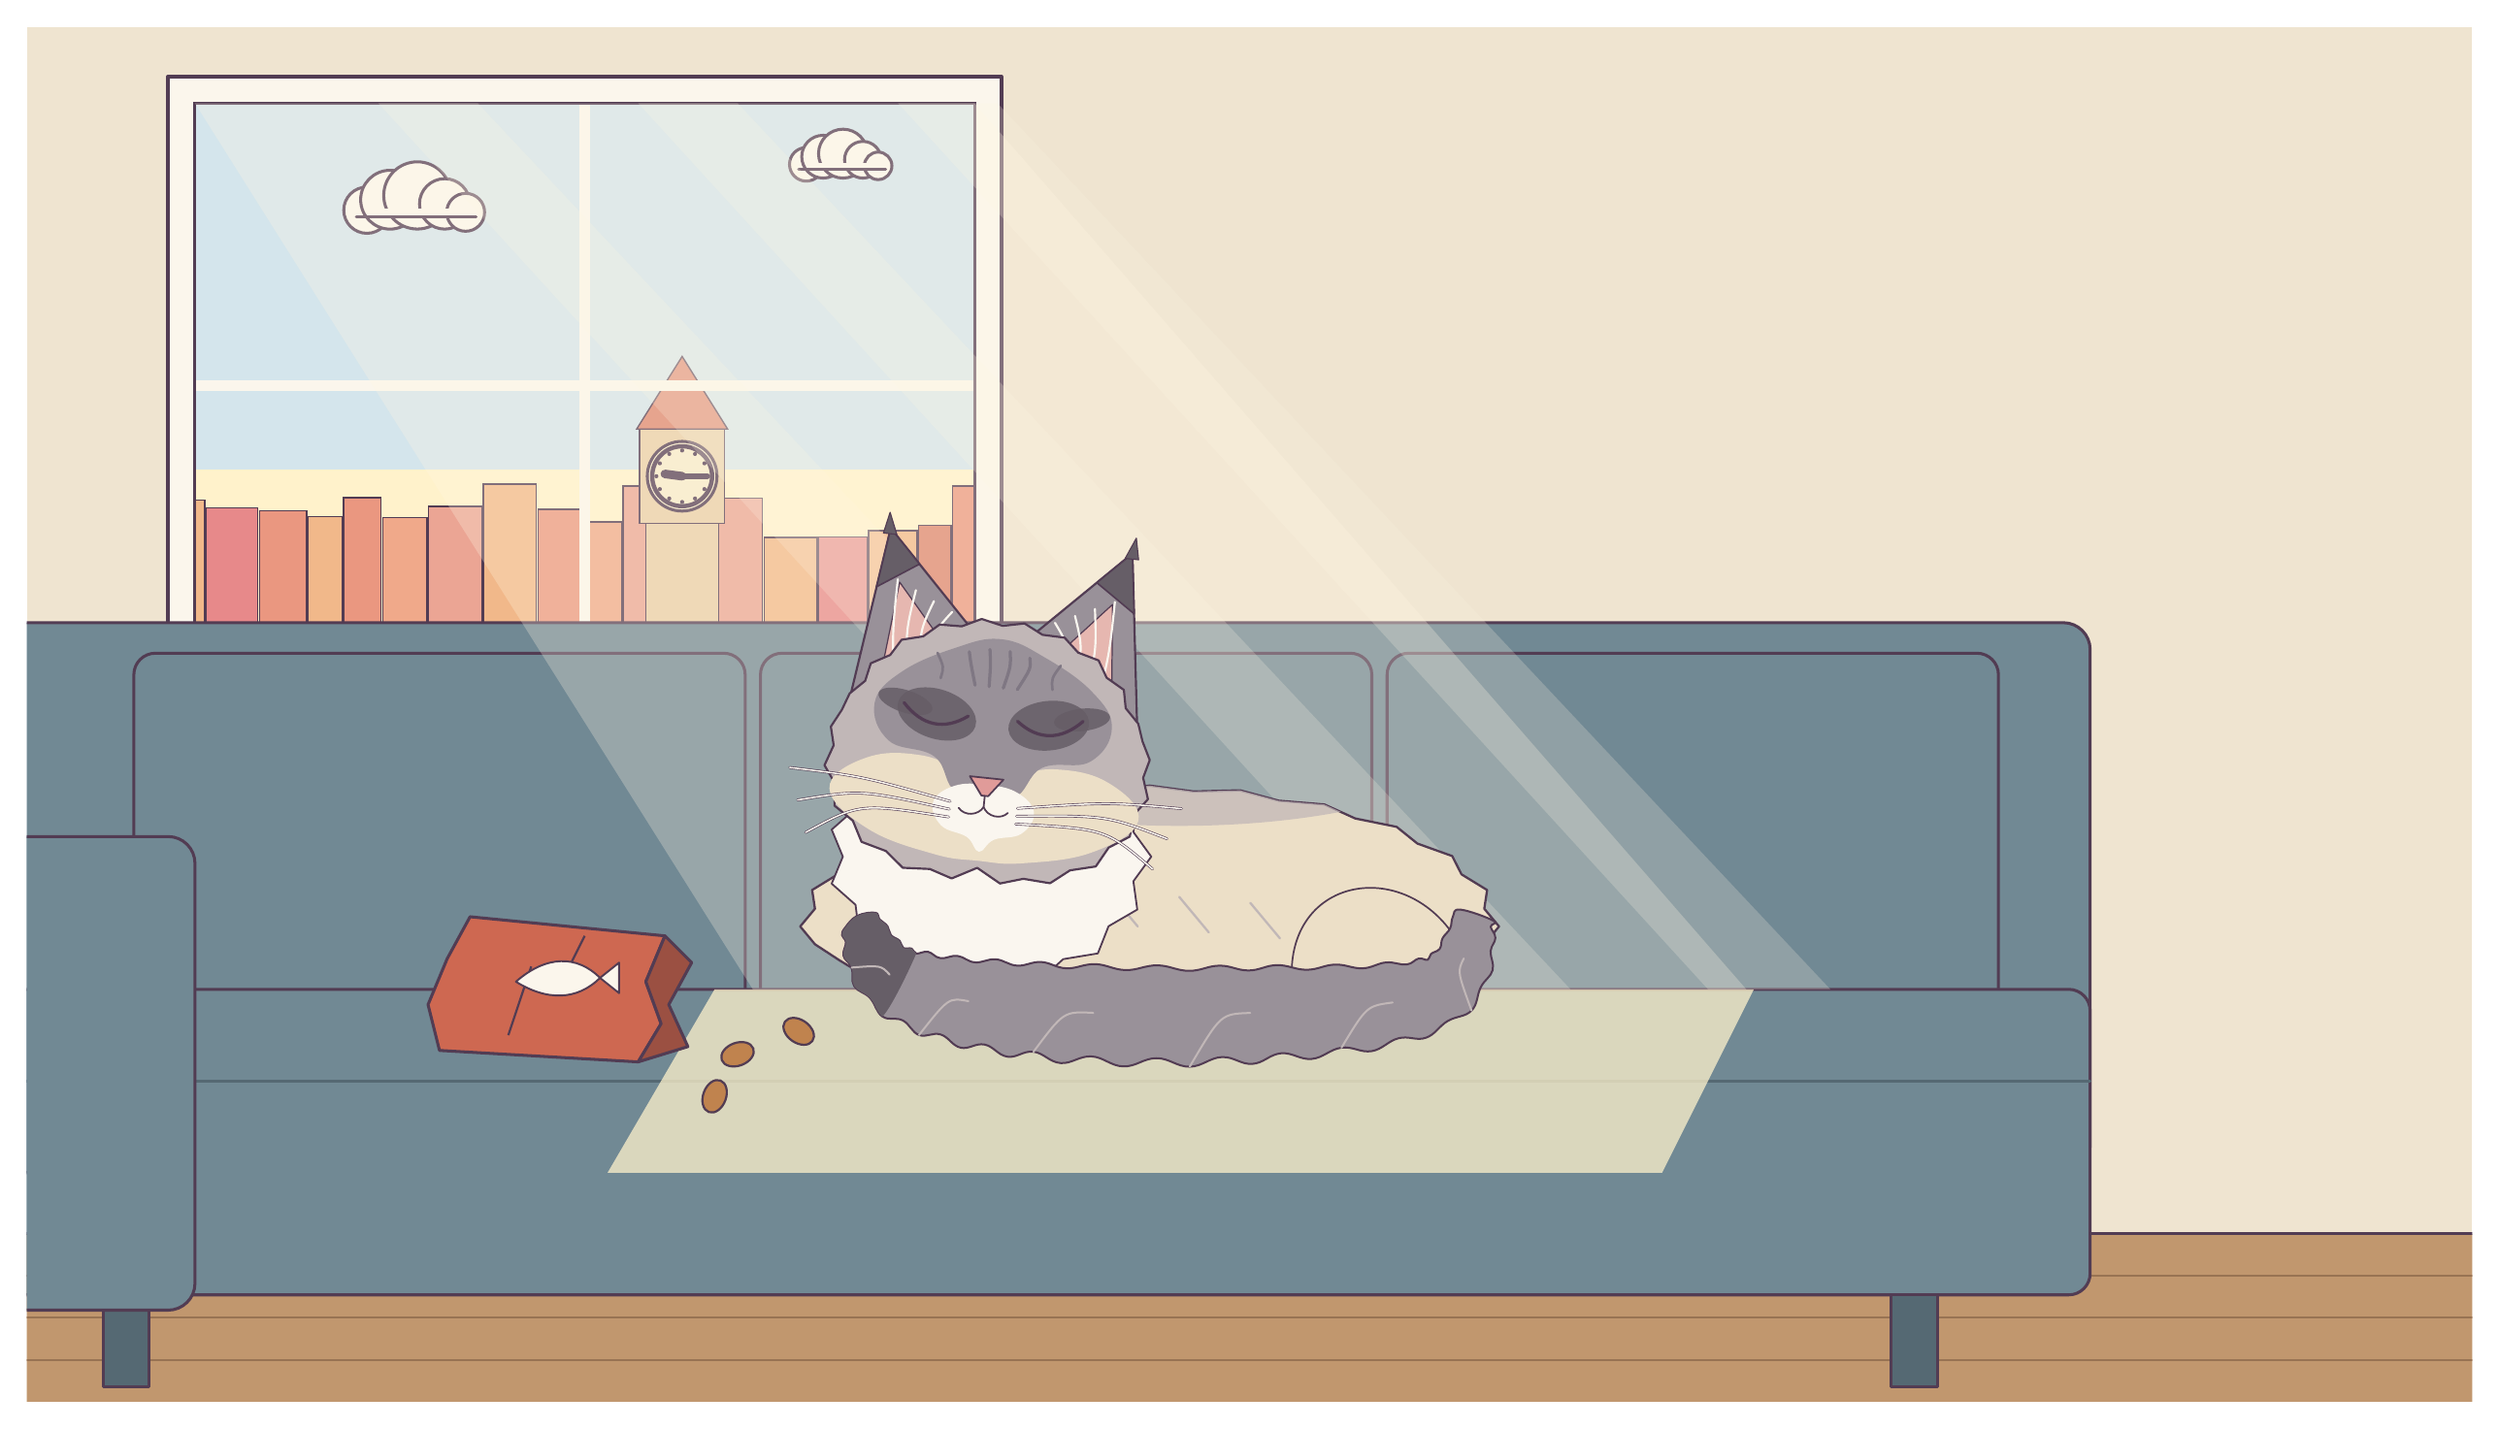
\begin{tikzpicture}
\clip (0,0) rectangle (32,18);
\fill[homewall] (0,0) rectangle (32,18);
\filldraw[inked,line width=1.4pt,fill=hometrim] (1.85,9.25) rectangle (12.75,17.35);
\begin{scope}\clip (2.2,9.6) rectangle (12.4,17);
\fill[morningsky] (2.2,9.6) rectangle (12.4,17);
\fill[homewindow] (2.2,9.6) rectangle (12.4,12.2);
\filldraw[inked,fill=hometrim] (4.45,15.6) circle (0.303);
\filldraw[inked,fill=hometrim] (4.753,15.737) circle (0.385);
\filldraw[inked,fill=hometrim] (5.11,15.793) circle (0.44);
\filldraw[inked,fill=hometrim] (5.468,15.682) circle (0.33);
\filldraw[inked,fill=hometrim] (5.742,15.572) circle (0.248);
\fill[hometrim] (4.45,15.518) rectangle (5.742,15.627);
\draw[ink, line width=1.1pt, line cap=round] (4.312,15.518) -- (5.88,15.518);
\filldraw[inked,fill=hometrim] (10.2,16.2) circle (0.22);
\filldraw[inked,fill=hometrim] (10.42,16.3) circle (0.28);
\filldraw[inked,fill=hometrim] (10.68,16.34) circle (0.32);
\filldraw[inked,fill=hometrim] (10.94,16.26) circle (0.24);
\filldraw[inked,fill=hometrim] (11.14,16.18) circle (0.18);
\fill[hometrim] (10.2,16.14) rectangle (11.14,16.22);
\draw[ink, line width=1.1pt, line cap=round] (10.1,16.14) -- (11.24,16.14);
\filldraw[ink,line width=0.5pt,fill=wallD] (1.9,9.6) rectangle (2.327,11.803);
\filldraw[ink,line width=0.5pt,fill=wallC] (2.347,9.6) rectangle (3.023,11.703);
\filldraw[ink,line width=0.5pt,fill=wallA] (3.043,9.6) rectangle (3.662,11.663);
\filldraw[ink,line width=0.5pt,fill=wallD] (3.682,9.6) rectangle (4.126,11.59);
\filldraw[ink,line width=0.5pt,fill=wallA] (4.146,9.6) rectangle (4.635,11.838);
\filldraw[ink,line width=0.5pt,fill=wallB] (4.655,9.6) rectangle (5.235,11.572);
\filldraw[ink,line width=0.5pt,fill=wallF] (5.255,9.6) rectangle (5.955,11.723);
\filldraw[ink,line width=0.5pt,fill=wallD] (5.975,9.6) rectangle (6.668,12.013);
\filldraw[ink,line width=0.5pt,fill=wallA] (6.688,9.6) rectangle (7.279,11.685);
\filldraw[ink,line width=0.5pt,fill=wallB] (7.299,9.6) rectangle (7.784,11.519);
\filldraw[ink,line width=0.5pt,fill=wallF] (7.804,9.6) rectangle (8.486,11.99);
\filldraw[ink,line width=0.5pt,fill=wallC] (8.506,9.6) rectangle (9.032,11.733);
\filldraw[ink,line width=0.5pt,fill=wallF] (9.052,9.6) rectangle (9.628,11.826);
\filldraw[ink,line width=0.5pt,fill=wallD] (9.648,9.6) rectangle (10.333,11.315);
\filldraw[ink,line width=0.5pt,fill=wallC] (10.353,9.6) rectangle (10.993,11.323);
\filldraw[ink,line width=0.5pt,fill=wallD] (11.013,9.6) rectangle (11.649,11.406);
\filldraw[ink,line width=0.5pt,fill=wallE] (11.669,9.6) rectangle (12.095,11.475);
\filldraw[ink,line width=0.5pt,fill=wallA] (12.115,9.6) rectangle (12.608,11.989);
\filldraw[ink,line width=0.5pt,fill=stone] (8.1,9.6) rectangle (9.05,11.5);
\filldraw[ink,line width=0.5pt,fill=stone] (8.02,11.5) rectangle (9.13,12.735);
\filldraw[inked,fill=clock] (8.575,12.117) circle (0.456);
\draw[ink, line width=1.6pt] (8.575,12.117) circle (0.392);
\foreach \k in {0,...,11} { \fill[ink] ($(8.575,12.117)+(\k*30:0.337)$) circle (0.027); }
\draw[ink, line width=3.2pt, line cap=round] (8.575,12.117) -- (8.349,12.147);
\draw[ink, line width=2.2pt, line cap=round] (8.575,12.117) -- (8.903,12.117);
\filldraw[inked,fill=ink] (8.575,12.117) circle (0.032);
\filldraw[ink,line width=0.5pt,fill=wallE] (7.98,12.735) -- (9.17,12.735) -- (8.575,13.685) -- cycle;
\end{scope}
\draw[hometrim, line width=4pt, line cap=round] (7.3,9.6) -- (7.3,17);
\draw[hometrim, line width=4pt, line cap=round] (2.2,13.3) -- (12.4,13.3);
\draw[ink, line width=1.1pt] (2.2,9.6) rectangle (12.4,17);
\filldraw[inked,fill=homefloor] (-0.5,-0.5) rectangle (32.5,2.2);
\draw[homefloordark, line width=0.7pt, line cap=round] (-0.5,0.55) -- (32.5,0.55);
\draw[homefloordark, line width=0.7pt, line cap=round] (-0.5,1.1) -- (32.5,1.1);
\draw[homefloordark, line width=0.7pt, line cap=round] (-0.5,1.65) -- (32.5,1.65);
\filldraw[inked,fill=sofa,rounded corners=10pt] (-1,3.0) rectangle (27,10.2);
\filldraw[inked,fill=sofa,rounded corners=8pt] (1.4,5) rectangle (9.4,9.8);
\filldraw[inked,fill=sofa,rounded corners=8pt] (9.6,5) rectangle (17.6,9.8);
\filldraw[inked,fill=sofa,rounded corners=8pt] (17.8,5) rectangle (25.8,9.8);
\filldraw[inked,fill=sofa,rounded corners=8pt] (-1,1.4) rectangle (27,5.4);
\draw[sofadark, line width=1.0pt, line cap=round] (-1,4.2) -- (27,4.2);
\filldraw[inked,fill=sofadark] (1.0,0.2) rectangle (1.6,1.4);
\filldraw[inked,fill=sofadark] (24.4,0.2) rectangle (25.0,1.4);
\filldraw[inked,fill=sofa,rounded corners=10pt] (-1,1.2) rectangle (2.2,7.4);
\fill[sunlight, opacity=0.28] (2.2,17) -- (12.4,17) -- (22.5,5.4) -- (9.5,5.4) -- cycle;
\fill[sunlight, opacity=0.22] (4.6,17) -- (5.9,17) -- (16.8,5.4) -- (15.2,5.4) -- cycle;
\fill[sunlight, opacity=0.22] (8,17) -- (9.3,17) -- (20.2,5.4) -- (18.6,5.4) -- cycle;
\fill[sunlight, opacity=0.22] (11.4,17) -- (12.7,17) -- (23.6,5.4) -- (22,5.4) -- cycle;
\fill[homewindow, opacity=0.75] (9.0,5.4) -- (22.6,5.4) -- (21.4,3.0) -- (7.6,3.0) -- cycle;
\filldraw[inked,fill=treatbag] (5.4,4.6) -- (8,4.45) -- (8.3,4.95) -- (8.1,5.5) -- (8.35,6.1) -- (5.8,6.35) -- (5.5,5.8) -- (5.25,5.2) -- cycle;
\filldraw[inked,fill=treatbagdark] (8,4.45) -- (8.65,4.65) -- (8.4,5.2) -- (8.7,5.75) -- (8.35,6.1) -- (8.1,5.5) -- (8.3,4.95) -- cycle;
\draw[ink, line width=0.8pt] (6.3,4.8) -- (6.6,5.7);
\draw[ink, line width=0.8pt] (7.3,6.1) -- (7,5.5);
\filldraw[inked,fill=hometrim,line width=0.7pt] (6.4,5.5) .. controls (6.8,5.85) and (7.2,5.85) .. (7.5,5.55) -- (7.75,5.75) -- (7.75,5.35) -- (7.5,5.55) .. controls (7.2,5.25) and (6.8,5.25) .. cycle;
\filldraw[inked,fill=treat,line width=0.8pt,rotate around={20:(9.3,4.55)}] (9.3,4.55) ellipse (0.22 and 0.15);
\filldraw[inked,fill=treat,line width=0.8pt,rotate around={-35:(10.1,4.85)}] (10.1,4.85) ellipse (0.22 and 0.15);
\filldraw[inked,fill=treat,line width=0.8pt,rotate around={70:(9,4)}] (9,4) ellipse (0.22 and 0.15);
\filldraw[inked,fill=catcream,line width=0.827pt] (19.265,6.223) -- (19.072,6.455) -- (19.109,6.7) -- (18.774,6.905) -- (18.652,7.145) -- (18.197,7.308) -- (17.925,7.527) -- (17.382,7.637) -- (16.979,7.82) -- (16.383,7.869) -- (15.876,8.005) -- (15.269,7.99) -- (14.692,8.067) -- (14.116,7.99) -- (13.509,8.005) -- (13.002,7.869) -- (12.406,7.82) -- (12.003,7.637) -- (11.46,7.527) -- (11.188,7.308) -- (10.733,7.145) -- (10.611,6.905) -- (10.276,6.7) -- (10.313,6.455) -- (10.12,6.223) -- (10.313,5.99) -- (10.629,5.783) -- (10.938,5.595) -- (11.05,5.374) -- (11.468,5.224) -- (11.718,5.022) -- (12.218,4.921) -- (12.589,4.753) -- (13.137,4.707) -- (13.604,4.583) -- (14.162,4.597) -- (14.692,4.525) -- (15.223,4.597) -- (15.781,4.583) -- (16.248,4.707) -- (16.796,4.753) -- (17.167,4.921) -- (17.667,5.022) -- (17.917,5.224) -- (18.335,5.374) -- (18.447,5.595) -- (18.756,5.783) -- (19.072,5.99) -- cycle;
\begin{scope}\clip (19.265,6.223) -- (19.072,6.455) -- (19.109,6.7) -- (18.774,6.905) -- (18.652,7.145) -- (18.197,7.308) -- (17.925,7.527) -- (17.382,7.637) -- (16.979,7.82) -- (16.383,7.869) -- (15.876,8.005) -- (15.269,7.99) -- (14.692,8.067) -- (14.116,7.99) -- (13.509,8.005) -- (13.002,7.869) -- (12.406,7.82) -- (12.003,7.637) -- (11.46,7.527) -- (11.188,7.308) -- (10.733,7.145) -- (10.611,6.905) -- (10.276,6.7) -- (10.313,6.455) -- (10.12,6.223) -- (10.313,5.99) -- (10.629,5.783) -- (10.938,5.595) -- (11.05,5.374) -- (11.468,5.224) -- (11.718,5.022) -- (12.218,4.921) -- (12.589,4.753) -- (13.137,4.707) -- (13.604,4.583) -- (14.162,4.597) -- (14.692,4.525) -- (15.223,4.597) -- (15.781,4.583) -- (16.248,4.707) -- (16.796,4.753) -- (17.167,4.921) -- (17.667,5.022) -- (17.917,5.224) -- (18.335,5.374) -- (18.447,5.595) -- (18.756,5.783) -- (19.072,5.99) -- cycle;
\fill[catpointlight, opacity=0.75] (15.08,8.78) ellipse (4.03 and 1.24);
\end{scope}
\draw[ink, line width=0.62pt] (16.63,5.06) .. controls (16.165,6.765) and (17.87,7.23) .. (18.645,6.145);
\draw[catpointlight, line width=0.827pt, line cap=round] (14.15,6.688) -- (14.537,6.223);
\draw[catpointlight, line width=0.827pt, line cap=round] (15.08,6.61) -- (15.467,6.145);
\draw[catpointlight, line width=0.827pt, line cap=round] (16.01,6.532) -- (16.398,6.067);
\filldraw[inked,fill=catwhite,line width=0.661pt] (14.714,7.137) -- (14.48,7.459) -- (14.531,7.83) -- (14.155,8.048) -- (14.015,8.404) -- (13.561,8.479) -- (13.253,8.759) -- (12.801,8.679) -- (12.379,8.833) -- (12.006,8.611) -- (11.543,8.614) -- (11.314,8.289) -- (10.89,8.139) -- (10.844,7.767) -- (10.532,7.491) -- (10.678,7.137) -- (10.532,6.783) -- (10.844,6.507) -- (10.89,6.135) -- (11.314,5.985) -- (11.543,5.66) -- (12.006,5.663) -- (12.379,5.441) -- (12.801,5.595) -- (13.253,5.515) -- (13.561,5.795) -- (14.015,5.87) -- (14.155,6.226) -- (14.531,6.444) -- (14.48,6.815) -- cycle;
\filldraw[inked,fill=catpoint,line width=0.723pt] plot[smooth cycle, tension=0.7] coordinates {(19.191,6.298) (19.156,6.219) (19.217,6.073) (19.155,5.899) (19.181,5.651) (19.027,5.43) (18.905,5.122) (18.591,4.984) (18.308,4.766) (17.951,4.76) (17.599,4.591) (17.203,4.636) (16.814,4.489) (16.414,4.563) (16.036,4.424) (15.637,4.513) (15.217,4.387) (14.784,4.499) (14.349,4.391) (13.931,4.522) (13.527,4.435) (13.173,4.583) (12.832,4.518) (12.532,4.677) (12.219,4.636) (11.958,4.809) (11.675,4.802) (11.462,4.993) (11.196,5.044) (11.033,5.288) (10.826,5.443) (10.793,5.685) (10.686,5.84) (10.718,6.016) (10.667,6.109) (10.709,6.208) (10.864,6.361) (11.103,6.403) (11.155,6.319) (11.262,6.227) (11.307,6.11) (11.422,6.035) (11.468,5.942) (11.579,5.933) (11.639,5.869) (11.793,5.891) (11.954,5.808) (12.178,5.837) (12.405,5.753) (12.679,5.793) (12.96,5.71) (13.273,5.758) (13.604,5.675) (13.981,5.73) (14.379,5.652) (14.794,5.714) (15.208,5.642) (15.608,5.71) (15.989,5.647) (16.362,5.717) (16.75,5.656) (17.121,5.724) (17.479,5.675) (17.785,5.752) (18.055,5.725) (18.212,5.803) (18.332,5.786) (18.374,5.863) (18.489,5.931) (18.525,6.067) (18.625,6.199) (18.66,6.348) (18.758,6.444)};
\begin{scope}\clip plot[smooth cycle, tension=0.7] coordinates {(19.191,6.298) (19.156,6.219) (19.217,6.073) (19.155,5.899) (19.181,5.651) (19.027,5.43) (18.905,5.122) (18.591,4.984) (18.308,4.766) (17.951,4.76) (17.599,4.591) (17.203,4.636) (16.814,4.489) (16.414,4.563) (16.036,4.424) (15.637,4.513) (15.217,4.387) (14.784,4.499) (14.349,4.391) (13.931,4.522) (13.527,4.435) (13.173,4.583) (12.832,4.518) (12.532,4.677) (12.219,4.636) (11.958,4.809) (11.675,4.802) (11.462,4.993) (11.196,5.044) (11.033,5.288) (10.826,5.443) (10.793,5.685) (10.686,5.84) (10.718,6.016) (10.667,6.109) (10.709,6.208) (10.864,6.361) (11.103,6.403) (11.155,6.319) (11.262,6.227) (11.307,6.11) (11.422,6.035) (11.468,5.942) (11.579,5.933) (11.639,5.869) (11.793,5.891) (11.954,5.808) (12.178,5.837) (12.405,5.753) (12.679,5.793) (12.96,5.71) (13.273,5.758) (13.604,5.675) (13.981,5.73) (14.379,5.652) (14.794,5.714) (15.208,5.642) (15.608,5.71) (15.989,5.647) (16.362,5.717) (16.75,5.656) (17.121,5.724) (17.479,5.675) (17.785,5.752) (18.055,5.725) (18.212,5.803) (18.332,5.786) (18.374,5.863) (18.489,5.931) (18.525,6.067) (18.625,6.199) (18.66,6.348) (18.758,6.444)};
\fill[catpointdark] plot[smooth cycle, tension=0.7] coordinates {(11.196,5.044) (11.033,5.288) (10.826,5.443) (10.793,5.685) (10.686,5.84) (10.718,6.016) (10.667,6.109) (10.709,6.208) (10.864,6.361) (11.103,6.403) (11.155,6.319) (11.262,6.227) (11.307,6.11) (11.422,6.035) (11.468,5.942) (11.579,5.933) (11.639,5.869)};
\end{scope}
\draw[catpointlight, line width=0.723pt, line cap=round] (18.804,5.804) .. controls (18.719,5.634) .. (18.905,5.122);
\draw[catpointlight, line width=0.723pt, line cap=round] (17.873,5.228) .. controls (17.533,5.182) .. (17.203,4.636);
\draw[catpointlight, line width=0.723pt, line cap=round] (16.01,5.091) .. controls (15.623,5.078) .. (15.217,4.387);
\draw[catpointlight, line width=0.723pt, line cap=round] (13.955,5.092) .. controls (13.569,5.112) .. (13.173,4.583);
\draw[catpointlight, line width=0.723pt, line cap=round] (12.321,5.245) .. controls (12.062,5.293) .. (11.675,4.802);
\draw[catpointlight, line width=0.723pt, line cap=round] (11.29,5.593) .. controls (11.176,5.715) .. (10.793,5.685);
\begin{scope}[rotate around={-6:(12.6,8.547)}]
\filldraw[inked,fill=catpoint,line width=0.785pt] (10.686,8.842) -- (12.335,9.946) -- (11.01,11.286) -- cycle;
\filldraw[inked,fill=catpointdark,line width=0.589pt] (10.906,10.504) -- (11.01,11.286) -- (11.434,10.858) -- cycle;
\filldraw[inked,fill=catear,line width=0.442pt] (11.057,9.124) -- (11.2,10.595) -- (11.964,9.731) -- cycle;
\draw[catwhite, line width=0.785pt, line cap=round] (11.775,9.394) .. controls (11.702,9.983) .. (11.923,10.278);
\draw[catwhite, line width=0.785pt, line cap=round] (11.599,9.394) .. controls (11.525,9.983) .. (11.672,10.395);
\draw[catwhite, line width=0.785pt, line cap=round] (11.422,9.394) .. controls (11.348,9.983) .. (11.422,10.513);
\draw[catwhite, line width=0.785pt, line cap=round] (11.245,9.394) .. controls (11.172,9.983) .. (11.172,10.631);
\filldraw[inked,fill=catpointdark,line width=0.393pt] (10.921,11.213) -- (10.98,11.492) -- (11.098,11.213) -- cycle;
\filldraw[inked,fill=catpoint,line width=0.785pt] (14.514,8.842) -- (12.865,9.946) -- (14.19,11.286) -- cycle;
\filldraw[inked,fill=catpointdark,line width=0.589pt] (14.294,10.504) -- (14.19,11.286) -- (13.766,10.858) -- cycle;
\filldraw[inked,fill=catear,line width=0.442pt] (14.143,9.124) -- (14,10.595) -- (13.236,9.731) -- cycle;
\draw[catwhite, line width=0.785pt, line cap=round] (13.425,9.394) .. controls (13.498,9.983) .. (13.277,10.278);
\draw[catwhite, line width=0.785pt, line cap=round] (13.601,9.394) .. controls (13.675,9.983) .. (13.528,10.395);
\draw[catwhite, line width=0.785pt, line cap=round] (13.778,9.394) .. controls (13.852,9.983) .. (13.778,10.513);
\draw[catwhite, line width=0.785pt, line cap=round] (13.955,9.394) .. controls (14.028,9.983) .. (14.028,10.631);
\filldraw[inked,fill=catpointdark,line width=0.393pt] (14.102,11.213) -- (14.22,11.492) -- (14.279,11.213) -- cycle;
\filldraw[inked,fill=catpointlight,line width=0.785pt] (14.698,8.621) -- (14.578,8.854) -- (14.499,9.078) -- (14.314,9.263) -- (14.265,9.499) -- (14.024,9.634) -- (13.896,9.848) -- (13.619,9.922) -- (13.422,10.098) -- (13.131,10.105) -- (12.882,10.228) -- (12.6,10.167) -- (12.318,10.228) -- (12.069,10.105) -- (11.778,10.098) -- (11.581,9.922) -- (11.304,9.848) -- (11.176,9.634) -- (10.935,9.499) -- (10.886,9.263) -- (10.701,9.078) -- (10.622,8.854) -- (10.502,8.621) -- (10.564,8.381) -- (10.472,8.109) -- (10.635,7.885) -- (10.657,7.597) -- (10.917,7.425) -- (11.059,7.162) -- (11.389,7.076) -- (11.631,6.881) -- (11.985,6.902) -- (12.282,6.809) -- (12.6,6.982) -- (12.918,6.809) -- (13.215,6.902) -- (13.569,6.881) -- (13.811,7.076) -- (14.141,7.162) -- (14.283,7.425) -- (14.543,7.597) -- (14.565,7.885) -- (14.728,8.109) -- (14.636,8.381) -- cycle;
\fill[catcream] plot[smooth cycle, tension=0.7] coordinates {(12.6,8.179) (13.483,8.371) (14.22,8.253) (14.632,7.811) (14.072,7.34) (13.189,7.104) (12.6,7.075) (12.011,7.104) (11.127,7.34) (10.568,7.811) (10.98,8.253) (11.716,8.371)};
\fill[catpoint] plot[smooth cycle, tension=0.7] coordinates {(12.6,9.991) (13.189,9.814) (13.852,9.431) (14.161,8.989) (13.925,8.518) (13.307,8.371) (12.953,7.929) (12.247,7.929) (11.893,8.371) (11.275,8.518) (11.039,8.989) (11.348,9.431) (12.011,9.814)};
\draw[cattabby, line width=1.178pt, line cap=round] (12.202,9.784) .. controls (12.232,9.652) .. (12.322,9.357);
\draw[cattabby, line width=1.178pt, line cap=round] (12.467,9.843) .. controls (12.497,9.652) .. (12.507,9.357);
\draw[cattabby, line width=1.178pt, line cap=round] (12.733,9.843) .. controls (12.762,9.652) .. (12.693,9.357);
\draw[cattabby, line width=1.178pt, line cap=round] (12.998,9.784) .. controls (13.027,9.652) .. (12.878,9.357);
\draw[cattabby, line width=0.982pt, line cap=round] (11.79,9.726) .. controls (11.893,9.549) .. (11.864,9.402);
\draw[cattabby, line width=0.982pt, line cap=round] (13.41,9.726) .. controls (13.307,9.549) .. (13.336,9.402);
\fill[catpointdark, opacity=0.85, rotate around={-12:(11.864,8.93)}] (11.864,8.93) ellipse (0.53 and 0.324);
\fill[catpointdark, opacity=0.85, rotate around={-12:(11.864,8.93)}] (11.422,8.96) ellipse (0.368 and 0.147);
\draw[ink, line width=1.178pt, line cap=round] (12.276,8.945) .. controls (11.982,8.724) and (11.687,8.754) .. (11.422,9.033);
\fill[catpointdark, opacity=0.85, rotate around={12:(13.336,8.93)}] (13.336,8.93) ellipse (0.53 and 0.324);
\fill[catpointdark, opacity=0.85, rotate around={12:(13.336,8.93)}] (13.778,8.96) ellipse (0.368 and 0.147);
\draw[ink, line width=1.178pt, line cap=round] (12.924,8.945) .. controls (13.218,8.724) and (13.513,8.754) .. (13.778,9.033);
\fill[catwhite] plot[smooth cycle, tension=0.7] coordinates {(12.6,8.076) (13.012,8.017) (13.263,7.782) (13.13,7.487) (12.777,7.369) (12.6,7.193) (12.423,7.369) (12.07,7.487) (11.937,7.782) (12.188,8.017)};
\filldraw[inked,fill=catnose,line width=0.638pt] (12.379,8.165) -- (12.821,8.165) -- (12.644,7.929) -- (12.556,7.929) -- cycle;
\draw[ink, line width=0.638pt, line cap=round] (12.6,7.929) -- (12.6,7.782) .. controls (12.541,7.664) and (12.364,7.635) .. (12.276,7.738);
\draw[ink, line width=0.638pt, line cap=round] (12.6,7.782) .. controls (12.659,7.664) and (12.836,7.635) .. (12.924,7.738);
\draw[ink, line width=0.982pt, line cap=round] (12.158,7.811) .. controls (10.98,8.017) .. (10.023,8.032);
\draw[catwhite, line width=0.54pt, line cap=round] (12.158,7.811) .. controls (10.98,8.017) .. (10.023,8.032);
\draw[ink, line width=0.982pt, line cap=round] (12.158,7.708) .. controls (10.98,7.841) .. (10.17,7.62);
\draw[catwhite, line width=0.54pt, line cap=round] (12.158,7.708) .. controls (10.98,7.841) .. (10.17,7.62);
\draw[ink, line width=0.982pt, line cap=round] (12.158,7.605) .. controls (10.98,7.664) .. (10.318,7.208);
\draw[catwhite, line width=0.54pt, line cap=round] (12.158,7.605) .. controls (10.98,7.664) .. (10.318,7.208);
\draw[ink, line width=0.982pt, line cap=round] (13.042,7.811) .. controls (14.22,8.017) .. (15.177,8.032);
\draw[catwhite, line width=0.54pt, line cap=round] (13.042,7.811) .. controls (14.22,8.017) .. (15.177,8.032);
\draw[ink, line width=0.982pt, line cap=round] (13.042,7.708) .. controls (14.22,7.841) .. (15.03,7.62);
\draw[catwhite, line width=0.54pt, line cap=round] (13.042,7.708) .. controls (14.22,7.841) .. (15.03,7.62);
\draw[ink, line width=0.982pt, line cap=round] (13.042,7.605) .. controls (14.22,7.664) .. (14.882,7.208);
\draw[catwhite, line width=0.54pt, line cap=round] (13.042,7.605) .. controls (14.22,7.664) .. (14.882,7.208);
\end{scope}
\fill[sunlight, opacity=0.12] (0,0) rectangle (32,18);
\end{tikzpicture}
\end{document}
